\chapter{力制御と位置制御の統合}
\label{sec:IntegrationControl}
本章では,力制御と位置制御を統合した油圧シリンダの制御を行う.
本制御で実現する動作を\figname\ref{fig5:forceandpositionIMAGE}に示す.
\figname\ref{fig5:forceandpositionIMAGE}は位置目標として正弦波目標を与えており,対象物(固定板)に触れていない時は位置目標に従い,対象物に触れたら力制御を行うことを目的とする.
実験機は\figname\ref{fig:Integ_system}にしめすようになっており,およそ\SI{85}{mm}の位置に固定板が取り付けてある.

\begin{figure}[t]
    \centering
        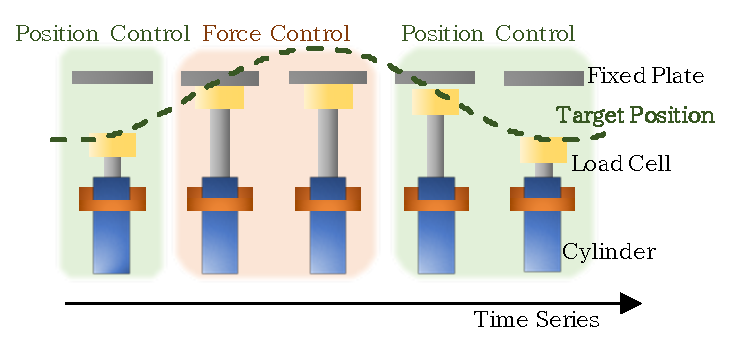
\includegraphics[keepaspectratio, scale=.9]{contents/IntegrationControl/figure/forceandpositionIMAGE.pdf}
        \caption{Image of Integration Control of Foce and Position}
        \label{fig5:forceandpositionIMAGE}
\end{figure}
\begin{figure}[t]
    \centering
        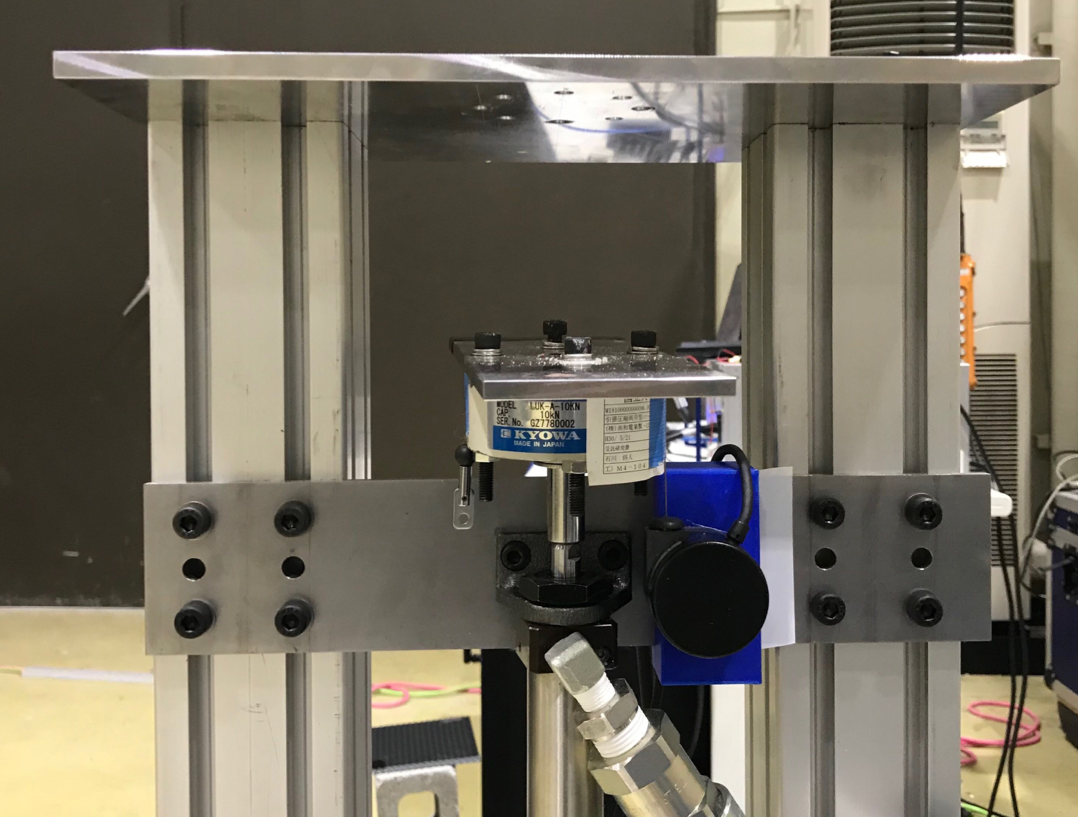
\includegraphics[keepaspectratio, width = .6\linewidth]{contents/IntegrationControl/figure/Integ_system.png}
        \caption{State of Cylinder Tip when Integration Control}
        \label{fig:Integ_system}
\end{figure}

制御にあたっては,(ⅰ)対象物に触れている時には力制御,それ以外には位置制御を行うというように力制御と位置制御を切り替える並列型の手法,(ⅱ)位置制御のからの入力をトルク入力と捉え,そのトルクを満たすように力制御を行う直列型の手法が考えられる.
並列型の手法では位置制御および力制御それぞれで設計した制御系をそのまま用いることができるという利点,直列型の手法ではコンプライアンス制御を行える利点がある.
そこで本章では並列型と直列型それぞれについて述べる.

\section{並列型制御手法}
\label{sec:並列型制御手法}
並列型の手法の概略を\figname\ref{fig5:pararell_torqueandposition}に示す.
位置制御はPD制御で行い,Pゲインを15,Dゲインを0.1とした.
また,力制御はPID制御,I-PD制御,サーボ系$H_\infty$制御により行い,PID制御とI-PD制御のゲインはPゲイン8.4,Iゲイン168,Dゲイン0.1とし,サーボ系$H_\infty$の制御器にはむだ時間を無視して設計したコントローラ$K_{H_\infty\mathrm{servo}}$を用いる.
力制御と位置制御の切り替えは,以下のアルゴリズムにより行う.
\begin{itembox}[l]{切り替えアルゴリズム}
    \begin{enumerate}
        \item ロッド先端が対象物に触れていない場合は位置制御を行う.
        \item 対象物に触れており,かつ力目標による力の付加方向と位置目標による進行方向が``一致している''場合は力制御を行う.
        \item 対象物に触れており,かつ力目標による力の付加方向と位置目標による進行方向が``逆''の場合は位置制御を行う.
    \end{enumerate}
\end{itembox}

また,接触非接触の判定は\figname\ref{fig5:touch_define}に示すように,目標値に対する割合で判定を行う.
非接触から接触と接触から非接触の閾値が異なるのは,チャタリングを防ぐためである.
また,制御モードが切り替わった際には積分器のリセットを行っている.

\begin{figure}[t]
    \centering
        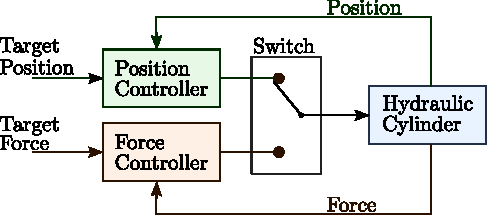
\includegraphics[keepaspectratio, scale=1.0]{contents/IntegrationControl/figure/pararell_torqueandposition.pdf}
        \caption{Force and Position Controller (Parallel)}
        \label{fig5:pararell_torqueandposition}
\end{figure}

\begin{figure}[t]
    \centering
        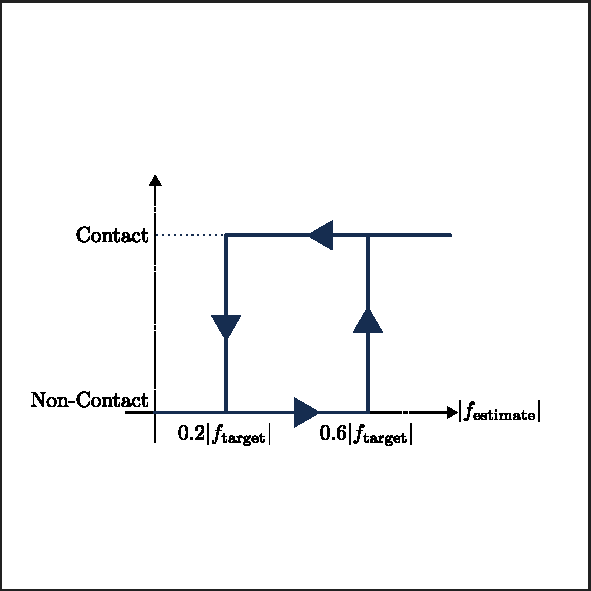
\includegraphics[keepaspectratio, scale=1.0]{contents/IntegrationControl/figure/touch_define.pdf}
        \caption{Decision of Touch or No Touch}
        \label{fig5:touch_define}
\end{figure}

力目標値として\SI{1}{kN},位置目標として振幅\SI{20}{mm},角振動数\SI{1}{rad/s}の正弦波を与える.
応答を\figname\ref{fig5:crop-FBsw_PID}から\figname\ref{fig5:crop-FBsw_JFPS4}に示す.
各グラフの(a)が力の応答,(b)が位置の応答を示しており,固定板は\SI{85}{mm}から\SI{90}{mm}付近に設置をしている.
I-PD制御(\figname\ref{fig5:crop-FBsw_IPD})において力制御時に応答が振動的になっているのは,オーバーシュート後の応答において$\fest$が小さくなりすぎ,位置制御と力制御が頻繁に切り替わっているためである.
この要因については,押し付け時に積分器をリセットしていることが影響していると考えられるが,本研究においてその検証までは至っていない.

\begin{figure}[t]
    \begin{minipage}{\minipageratio\hsize}
    \centering
        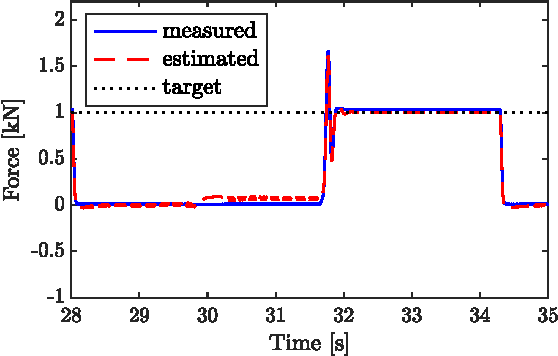
\includegraphics[keepaspectratio, scale = \minifigscale]{contents/IntegrationControl/figure/SECASQ/crop-FBsw_PID_force.pdf}
        \subcaption{$\fmsr$ and $\fest$}
        \label{fig5:crop-FBsw_PID_force}
    \end{minipage}
    \begin{minipage}{\minipageratio\hsize}
    \centering
        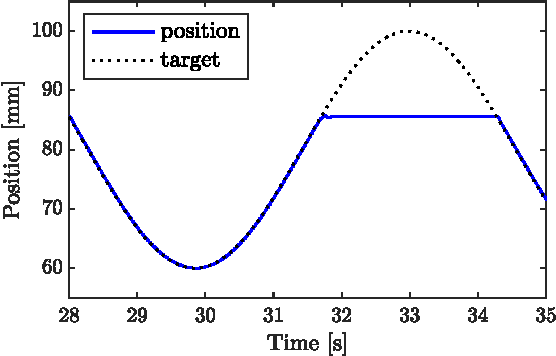
\includegraphics[keepaspectratio, scale = \minifigscale]
        {contents/IntegrationControl/figure/SECASQ/crop-FBsw_PID_pos.pdf}
        \subcaption{Position}
        \label{fig5:crop-FBsw_PID_pos}
    \end{minipage}
    \caption{Parallel Control (Position Controller: PD, Force Controller: PID)}   
    \label{fig5:crop-FBsw_PID}
\end{figure}

\begin{figure}[t]
    \begin{minipage}{\minipageratio\hsize}
    \centering
        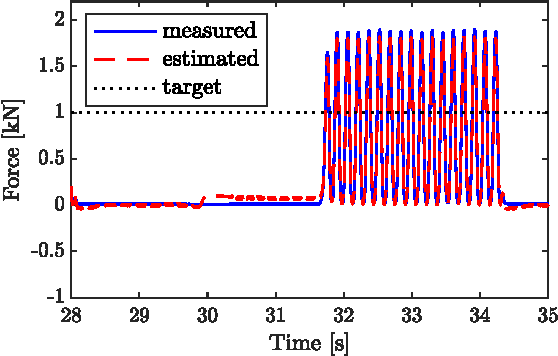
\includegraphics[keepaspectratio, scale = \minifigscale]{contents/IntegrationControl/figure/SECASQ/crop-FBsw_IPD_force.pdf}
        \subcaption{$\fmsr$ and $\fest$}
        \label{fig5:crop-FBsw_IPD_force}
    \end{minipage}
    \begin{minipage}{\minipageratio\hsize}
    \centering
        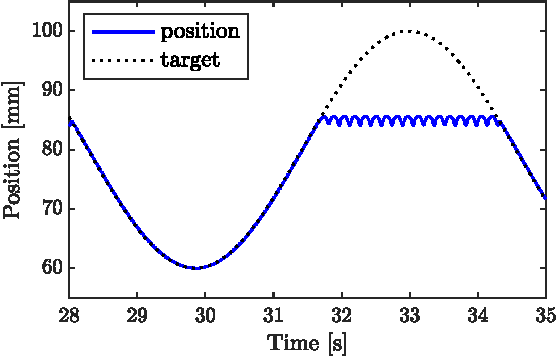
\includegraphics[keepaspectratio, scale = \minifigscale]
        {contents/IntegrationControl/figure/SECASQ/crop-FBsw_IPD_pos.pdf}
        \subcaption{Position}
        \label{fig5:crop-FBsw_IPD_pos}
    \end{minipage}
    \caption{Parallel Control (Position Controller: PD, Force Controller: I-PD)}
    \label{fig5:crop-FBsw_IPD}
\end{figure}

\begin{figure}[t]
    \begin{minipage}{\minipageratio\hsize}
    \centering
        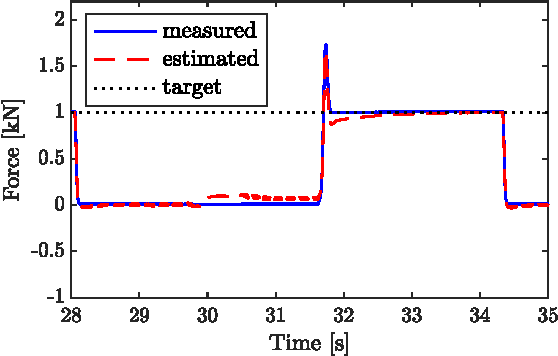
\includegraphics[keepaspectratio, scale = \minifigscale]{contents/IntegrationControl/figure/SECASQ/crop-FBsw_JFPS4_force.pdf}
        \subcaption{$\fmsr$ and $\fest$}
        \label{fig5:crop-FBsw_JFPS4_force}
    \end{minipage}
    \begin{minipage}{\minipageratio\hsize}
    \centering
        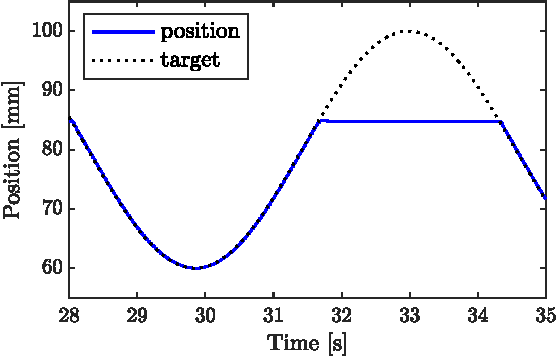
\includegraphics[keepaspectratio, scale = \minifigscale]
        {contents/IntegrationControl/figure/SECASQ/crop-FBsw_JFPS4_pos.pdf}
        \subcaption{Position}
        \label{fig5:crop-FBsw_JFPS4_pos}
    \end{minipage}
    \caption{Parallel Control (Position Controller: PD, Force Controller: $K_{H_\infty\mathrm{servo}}$)}   
    \label{fig5:crop-FBsw_JFPS4}
\end{figure}
% \begin{figure}[t]
%     \begin{minipage}{\minipageratio\hsize}
%     \centering
%         \includegraphics[keepaspectratio, width = \minifigwidth]
%         \subcaption{}
%         \label{fig5:}
%     \end{minipage}
%     \begin{minipage}{\minipageratio\hsize}
%     \centering
%         \includegraphics[keepaspectratio, width = \minifigwidth]
%         \subcaption{}
%         \label{fig5:}
%     \end{minipage}
%     \caption{}   
%     \label{fig5:}
% \end{figure}

\newpage
\section{直列型制御手法}
直列型の手法の概略を\figname\ref{fig5:casquade_torqueandposition}に示す.
位置制御による入力をトルク入力とみなし,そのトルクを満たすように力制御を行うことにより位置の制御と力の制御を両立させる.
また,トルク入力値に制限を設けることにより,その制限値が力目標値となる.

\begin{figure}[t]
    \centering
        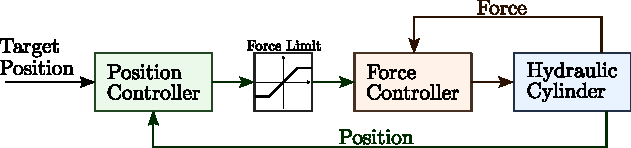
\includegraphics[keepaspectratio, scale = 1.0]{contents/IntegrationControl/figure/casquade_torqueandposition.pdf}
        \caption{Force and Position Controller (Cascade)}
        \label{fig5:casquade_torqueandposition}
\end{figure}

\subsection{位置制御ゲイン調整による直列型制御}
直列型の手法において,\ref{sec:並列型制御手法}節におけるそれぞれの制御器を直列につなぎ変えたのみでは位置制御器からの出力が小さく,位置制御の応答性が悪化する.
そこで位置制御器のゲインをPゲイン850,Dゲイン4とした.
そのときの応答を\figname\ref{fig5:crop-FBcsqtch_PID_Notrq_posPIDadjust}から\figname\ref{fig5:crop-FBcsqtch_JFPS4_Notrq_posPIDadjust}に示す.


\begin{figure}[t]
    \begin{minipage}{\minipageratio\hsize}
    \centering
        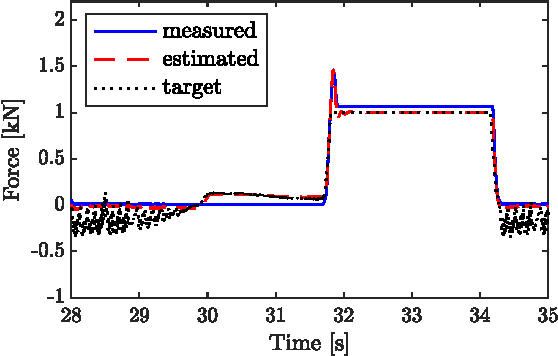
\includegraphics[keepaspectratio, scale = \minifigscale]{contents/IntegrationControl/figure/SECASQ/crop-FBcsqtch_PID_Notrq_posPIDadjust_force.pdf}
        \subcaption{$\fmsr$ and $\fest$}
        \label{fig5:crop-FBcsqtch_PID_Notrq_posPIDadjust_force}
    \end{minipage}
    \begin{minipage}{\minipageratio\hsize}
    \centering
        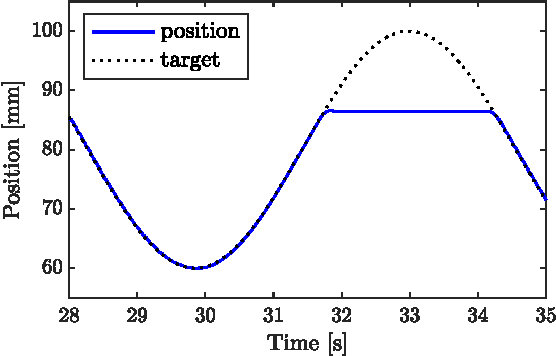
\includegraphics[keepaspectratio, scale = \minifigscale]{contents/IntegrationControl/figure/SECASQ/crop-FBcsqtch_PID_Notrq_posPIDadjust_pos.pdf}
        \subcaption{Position}
        \label{fig5:crop-FBcsqtch_PID_Notrq_posPIDadjust_pos}
    \end{minipage}
    \caption{Cascade Control (Position Controller: PD, Force Controller: PID)}  
    \label{fig5:crop-FBcsqtch_PID_Notrq_posPIDadjust}
\end{figure}

\begin{figure}[t]
    \begin{minipage}{\minipageratio\hsize}
    \centering
        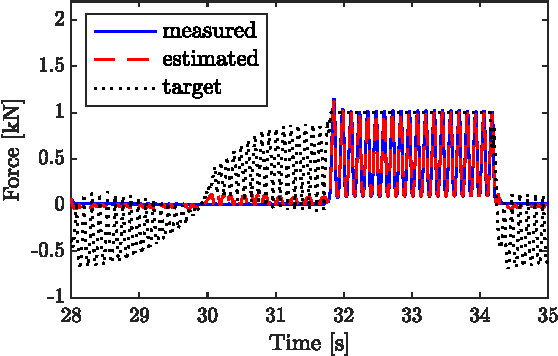
\includegraphics[keepaspectratio, scale = \minifigscale]{contents/IntegrationControl/figure/SECASQ/crop-FBcsqtch_IPD_Notrq_posPIDadjust_force.pdf}
        \subcaption{$\fmsr$ and $\fest$}
        \label{fig5:crop-FBcsqtch_IPD_Notrq_posPIDadjust_force}
    \end{minipage}
    \begin{minipage}{\minipageratio\hsize}
    \centering
        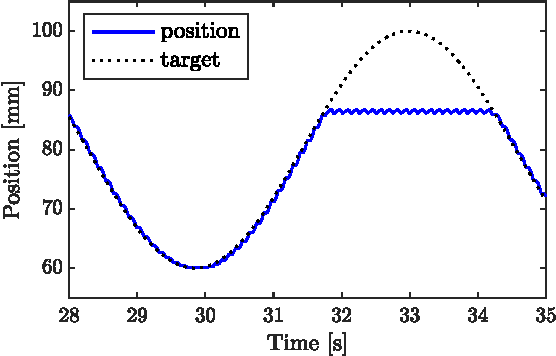
\includegraphics[keepaspectratio, scale = \minifigscale]{contents/IntegrationControl/figure/SECASQ/crop-FBcsqtch_IPD_Notrq_posPIDadjust_pos.pdf}
        \subcaption{Position}
        \label{fig5:crop-FBcsqtch_IPD_Notrq_posPIDadjust_pos}
    \end{minipage}
    \caption{Cascade Control (Position Controller: PD, Force Controller: I-PD)}  
    \label{fig5:crop-FBcsqtch_IPD_Notrq_posPIDadjust}
\end{figure}

\begin{figure}[t]
    \begin{minipage}{\minipageratio\hsize}
    \centering
        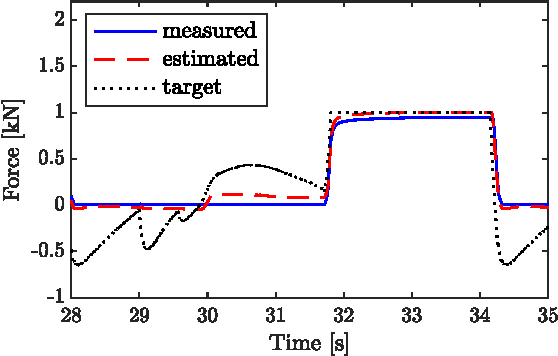
\includegraphics[keepaspectratio, scale = \minifigscale]{contents/IntegrationControl/figure/SECASQ/crop-FBcsqtch_JFPS4_Notrq_posPIDadjust_force.pdf}
        \subcaption{$\fmsr$ and $\fest$}
        \label{fig5:crop-FBcsqtch_JFPS4_Notrq_posPIDadjust_force}
    \end{minipage}
    \begin{minipage}{\minipageratio\hsize}
    \centering
        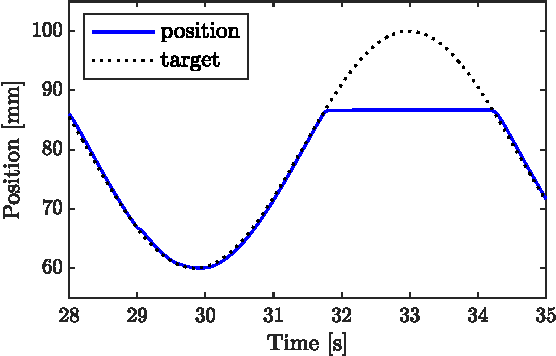
\includegraphics[keepaspectratio, scale = \minifigscale]{contents/IntegrationControl/figure/SECASQ/crop-FBcsqtch_JFPS4_Notrq_posPIDadjust_pos.pdf}
        \subcaption{Position}
        \label{fig5:crop-FBcsqtch_JFPS4_Notrq_posPIDadjust_pos}
    \end{minipage}
    \caption{Cascade Control (Position Controller: PD, Force Controller: $K_{H_\infty\mathrm{servo}}$)}  
    \label{fig5:crop-FBcsqtch_JFPS4_Notrq_posPIDadjust}
\end{figure}

\clearpage
\subsection{トルク補償による直列型制御}
次に位置制御のPDゲインを\ref{sec:並列型制御手法}節と同様にPゲイン15,Dゲイン0.1としたまま,トルク補償を行うことにより応答性の改善を図る.
トルク補償を行うことにより,位置制御のみを行って決定したゲインをそのまま統合制御に使用することが可能になると期待される.
位置制御におけるトルク補償の概要を\figname\ref{fig5:torque_compensator}に示す.
\figname\ref{fig5:torque_compensator}中の$\Delta T$はサンプリング時間,$m$はロッドとロードセルの合計質量である.
ロッドの質量は直接測定できなかったためカタログ値から推定し,合計質量は$m=1.2$とした.

\begin{figure}[t]
    \centering
        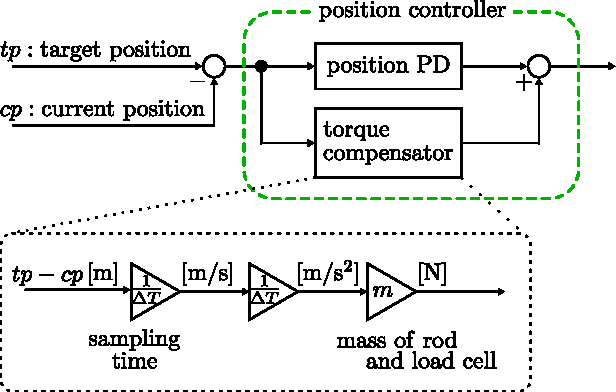
\includegraphics[keepaspectratio, scale=1.0]{contents/IntegrationControl/figure/torque_compensator.pdf}
        \caption{Torque Compensator}
        \label{fig5:torque_compensator}
\end{figure}

トルク補償による応答の結果を\figname\ref{fig5:crop-FBcsqtch_PID_trq}から\figname\ref{fig5:crop-FBcsqtch_JFPS4_trq}に示す.

\begin{figure}[t]
    \begin{minipage}{\minipageratio\hsize}
    \centering
        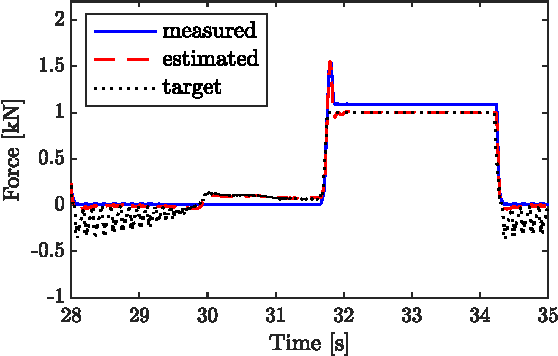
\includegraphics[keepaspectratio, scale = \minifigscale]{contents/IntegrationControl/figure/SECASQ/crop-FBcsqtch_PID_trq_force.pdf}
        \subcaption{$\fmsr$ and $\fest$}
        \label{fig5:crop-FBcsqtch_PID_trq_force}
    \end{minipage}
    \begin{minipage}{\minipageratio\hsize}
    \centering
        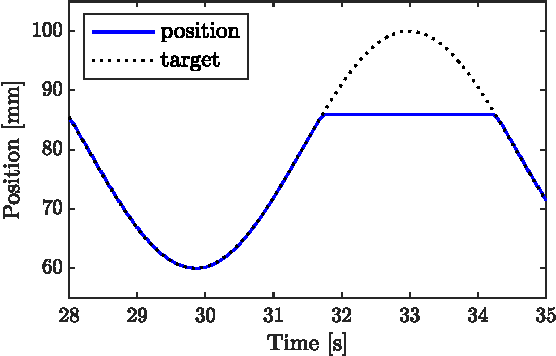
\includegraphics[keepaspectratio, scale = \minifigscale]{contents/IntegrationControl/figure/SECASQ/crop-FBcsqtch_PID_trq_pos.pdf}
        \subcaption{Position}
        \label{fig5:crop-FBcsqtch_PID_trq_pos}
    \end{minipage}
    \caption{Cascade Control (Position Controller: PD with Torque Compensate, Force Controller: PID)}  
    \label{fig5:crop-FBcsqtch_PID_trq}
\end{figure}

\begin{figure}[t]
    \begin{minipage}{\minipageratio\hsize}
    \centering
        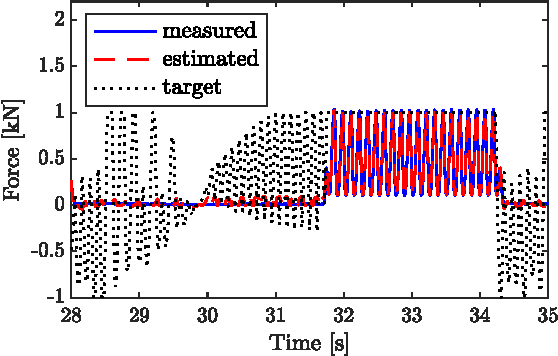
\includegraphics[keepaspectratio, scale = \minifigscale]{contents/IntegrationControl/figure/SECASQ/crop-FBcsqtch_IPD_trq_force.pdf}
        \subcaption{$\fmsr$ and $\fest$}
        \label{fig5:crop-FBcsqtch_IPD_trq_force}
    \end{minipage}
    \begin{minipage}{\minipageratio\hsize}
    \centering
        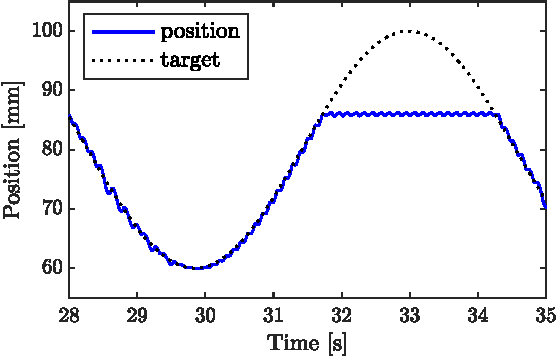
\includegraphics[keepaspectratio, scale = \minifigscale]{contents/IntegrationControl/figure/SECASQ/crop-FBcsqtch_IPD_trq_pos.pdf}
        \subcaption{Position}
        \label{fig5:crop-FBcsqtch_IPD_trq_pos}
    \end{minipage}
    \caption{Cascade Control (Position Controller: PD with Torque Compensate, Force Controller: I-PD)}  
    \label{fig5:crop-FBcsqtch_IPD_trq}
\end{figure}

\begin{figure}[t]
    \begin{minipage}{\minipageratio\hsize}
    \centering
        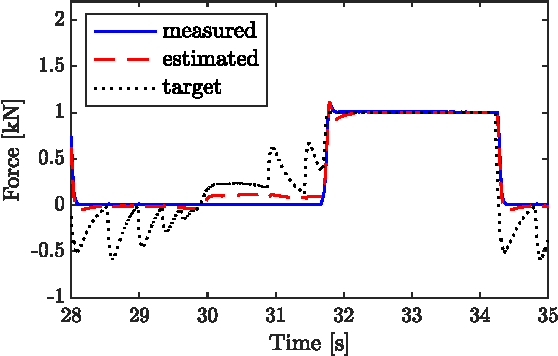
\includegraphics[keepaspectratio, scale = \minifigscale]{contents/IntegrationControl/figure/SECASQ/crop-FBcsqtch_JFPS4_trq_force.pdf}
        \subcaption{$\fmsr$ and $\fest$}
        \label{fig5:crop-FBcsqtch_JFPS4_trq_force}
    \end{minipage}
    \begin{minipage}{\minipageratio\hsize}
    \centering
        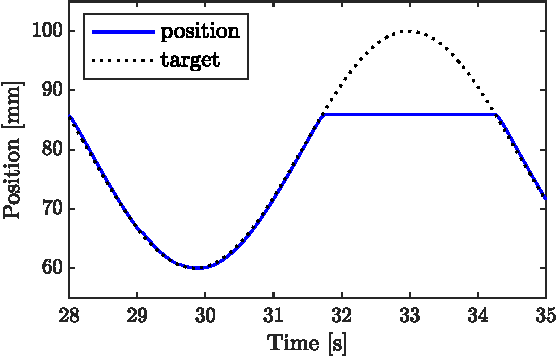
\includegraphics[keepaspectratio, scale = \minifigscale]{contents/IntegrationControl/figure/SECASQ/crop-FBcsqtch_JFPS4_trq_pos.pdf}
        \subcaption{Position}
        \label{fig5:crop-FBcsqtch_JFPS4_trq_pos}
    \end{minipage}
    \caption{Cascade Control (Position Controller: PD with Torque Compensate, Force Controller: $K_{H_\infty\mathrm{servo}}$)}  
    \label{fig5:crop-FBcsqtch_JFPS4_trq}
\end{figure}


\clearpage
\section{コンプライアンス制御}
コンプライアンス制御とは,アクチュエータの剛性を制御する手法である\cite{松野_大須賀_松原_野田_稲見201712,吉川198811,谷江和雄1989コンプライアンス制御と柔軟接触問題}.
多リンク系のマニピュレータにおいてはコンプライアンスにより,対象物に沿うように手先を押し付ける倣い操作が可能になる.
本研究で扱う油圧シリンダーにおいては構造上倣い操作はできないが,コンプライアンス制御においてアクチュエータの剛性を柔らかくできることを示す.
\subsection{外力と仮想バネ}
アクチュエータの運動方程式は\eqnname\eqref{eq:eom_of_rod}より
\begin{align}
    \label{eq:eom_of_compra}
    m\ddot{x_\mathrm{p}} + B\dot{x_\mathrm{p}} = \fout +F_\mathrm{ext}
\end{align}
と表せる.
$x_\mathrm{p}$はアクチュエータの位置,$\fout$はアクチュエータの出力,$m$はロッドとロードセルの合計質量,$B$は粘性項をまとめたものである\footnote{本来はここにクーロン摩擦も加わるが,本研究では考慮できていない.}.
ここで,位置の目標値$x_\mathrm{ref}$に対し,$\fout = k(x_\mathrm{ref}-x_\mathrm{p})$となるようにすると,\eqnname\eqref{eq:eom_of_compra}は
\begin{align}
    \label{eq:hoge}
    m\ddot{x_\mathrm{p}} + B\dot{x_\mathrm{p}} = k(x_\mathrm{ref}-x_\mathrm{p}) +F_\mathrm{ext}
\end{align}
となり,これは外力$F_\mathrm{ext}$を受けたバネマスダンパ系の運動方程式となる.
$k$を仮想バネ定数といい,$k$を変えることにより関節の剛性を変化させる制御のことをコンプライアンス制御という.

\subsection{コンプライアンス制御の応答とフィードバック変調器の導入}
位置目標値を\SI{80}{mm},仮想バネ定数$k$を5\SI{50}{N/mm}および\SI{100}{N/mm}に設定した時の位置の応答を\figname\ref{fig:compra_k50-crop}および\figname\ref{fig:compra_k100-crop}に青破線で示す.
荷重として\figname\ref{fig:omori}に示す\SI{15}{kg}のおもりを乗せる.
おもりを手作業でのせているためおおよその時間であるが,\SI{0}{s}から\SI{20}{s}および\SI{40}{s}から\SI{60}{s}までが荷重をかけていない状態,\SI{20}{s}から\SI{40}{s}までが荷重として\SI{15}{kg}のおもりをのせた時の応答である.
\figname\ref{fig:compra_k50-crop}および\figname\ref{fig:compra_k100-crop}において,荷重および仮想バネ定数に応じて位置が変位しており,コンプライアンス制御が機能していることが確認できる.
無負荷状態において目標値との間に偏差は摩擦による影響が大きいと考えられる.

\begin{figure}[t]
    \centering
        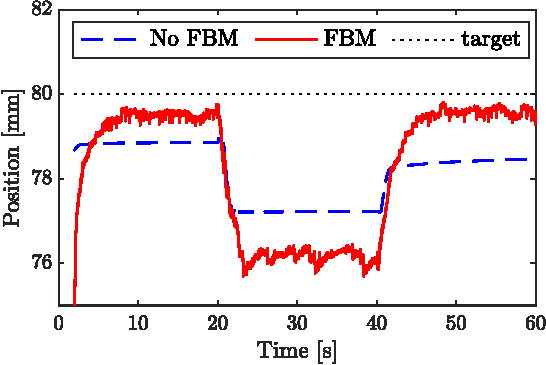
\includegraphics[keepaspectratio, scale=1.0]{contents/IntegrationControl/figure/compra/compra_k50-crop.pdf}
        \caption{Compliance Control (Virtual Stiffness $k=50$)}
        \label{fig:compra_k50-crop}
\end{figure}
\begin{figure}[t]
    \centering
        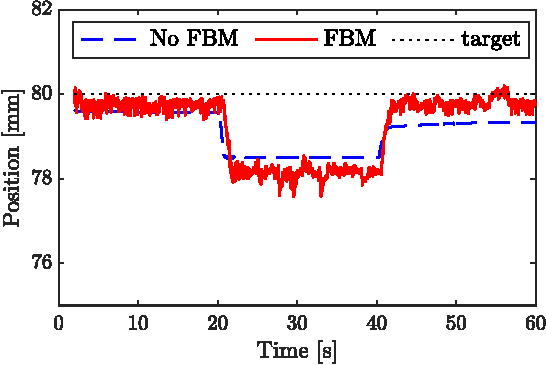
\includegraphics[keepaspectratio, scale=1.0]{contents/IntegrationControl/figure/compra/compra_k100-crop.pdf}
        \caption{Compliance Control (Virtual Stiffness $k=100$)}
        \label{fig:compra_k100-crop}
\end{figure}

\begin{figure}[t]
    \centering
        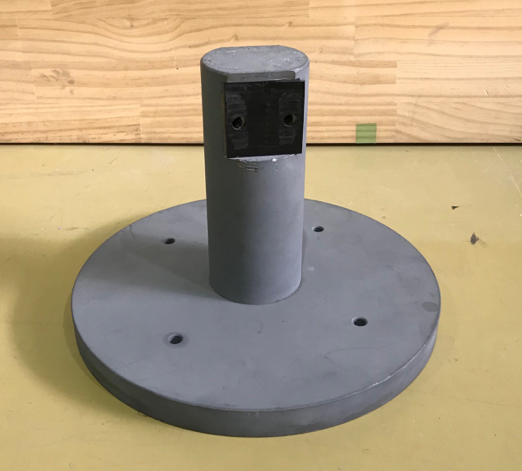
\includegraphics[keepaspectratio, width = .6\linewidth]{contents/IntegrationControl/figure/weigth.png}
        \caption{Weight(\SI{15}{kg})}
        \label{fig:omori}
\end{figure}

摩擦による定常偏差を減らすために,フィードバック変調器(Feedback Module;FBM)を導入する\footnote{定常偏差を解消する手法として積分器を導入する手法もあるが,コンプライアンス制御の特性上積分器の導入は難しい}\cite{石川将人2007,石川将人2008フィードバック変調器を用いた離散値入力制御におけるアクチュエータ非線形性の補償}.
FBMの詳細については付録\ref{sec:FBM}に譲るが,FBMとはフィードバックを有する量子化器の一つであり,コントローラからの入力値を時間的・空間的に離散化することによって切り替え速度の遅いアクチュエータへの対応や,摩擦の補償を行うことが可能である\cite{石川将人2008フィードバック変調器を用いた離散値入力制御におけるアクチュエータ非線形性の補償,佐藤順紀2013不等間隔量子化入力とアクチュエータの非線形要素モデルを用いたフィードバック変調器による油圧駆動システムの軌道制御,Ohgi_2008jrm}.
本研究ではFBMを\figname\ref{fig:casquade_torqueandposition_FBM}に示すように位置制御器と力制御器の間に挿入する.
力制御器の目標値をFBMで整形することにより,摩擦力を陽に考慮して空間量子化幅を設計することが可能である.
FBMのサンプリング時間\SI{0.02}{s},空間量子化幅0.5とした.
また,量子化誤差$\eta$からFBMの出力$u_\mathrm{Q}$までの雑音伝達関数$N(s)$を
\begin{align}
    \label{eq:Ns}
    N(s) = \left( \frac{0.022s}{0.022s+1} \right)^2
\end{align}
とした.
FBMを導入したときの位置の応答を\figname\ref{fig:compra_k50-crop}および\figname\ref{fig:compra_k100-crop}に赤の実線で示す.
これらより,FBMを用いない場合と比べて定常特性が改善されていることが確認できる.
\begin{figure}[t]
    \centering
        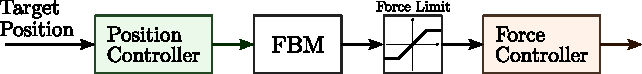
\includegraphics[keepaspectratio, scale=1.0]{contents/IntegrationControl/figure/casquade_torqueandposition_FBM.pdf}
        \caption{Cascade Controller with FBM}
        \label{fig:casquade_torqueandposition_FBM}
\end{figure}

無負荷状態(\SI{10}{s}から\SI{18}{s})および負荷状態(\SI{25}{s}から\SI{35}{s})での位置の平均値,および両者の差に仮想バネ定数を乗じた値について\tabname\ref{tab:position}に示す.
重りが\SI{15}{kg}であるため,重りによる外力は\SI{147}{N}となる.
よって\tabname\ref{tab:position}より,FBMを用いた場合において変位から計算される荷重と重りから受ける力の差が\SI{15}{N}となり,想定しているコンプライアンス制御の挙動に近くなり,FBMを導入した効果が現れていることが確認できる.

\begin{table}[t]
    \caption{Rod Position and Force}
    \label{tab:position}
    \centering
    \begin{tabular}{cccc}
    Virtual Stiffness&No Load [mm] &Loaded [mm] &$k(\mathrm{No~Load} - \mathrm{Load})$ [N]\\ \hline
        $k=50$&78.85&77.21&81.10\\
        $k=50$(with FBM)&79.51&76.22&164.6\\
        $k=100$&79.57&78.50&106.1\\
        $k=100$(with FBM)&79.74&78.13&161.5\\ \hline
    \end{tabular}
\end{table}
%\begin{figure}[t]
%    \begin{minipage}{\minipageratio\hsize}
%    \centering
%        \includegraphics[keepaspectratio, width = \minifigwidth]
%        \subcaption{}
%        \label{fig5:}
%    \end{minipage}
%    \begin{minipage}{\minipageratio\hsize}
%    \centering
%        \includegraphics[keepaspectratio, width = \minifigwidth]
%        \subcaption{}
%        \label{fig5:}
%    \end{minipage}
%    \caption{}   
%    \label{fig5:}
%\end{figure}
